\documentclass[25pt, a1paper, portrait,innermargin=15mm,
blockverticalspace=5mm, colspace=10mm, subcolspace=3mm]{tikzposter}
% font size: The size of the text in the main body may be set as : 12pt, 14pt, 17pt, 20pt, or 25pt;
% paper size: Currently, paper sizes may be set to : a0paper, a1paper, or a2paper;
% orientation: Either landscape or portrait
\usepackage[utf8]{inputenc}
\usepackage[T1]{fontenc}

\usepackage[ngerman]{babel}
\usepackage{pdfpages}
\usepackage{tikzpagenodes}

\usepackage{rustic}
\usepackage{lmodern}
%\usepackage[sfdefault,lf]{carlito}
\usepackage{fontawesome}
\usepackage{blindtext}
\usepackage{comment}
\usepackage{hyperref}
\usepackage{listings}

\usetheme{Simple}
%\usetitlestyle{Empty}\usebackgroundstyle{Empty}

%--------------------------------------
\usepackage[light,default]{raleway}

%-------------- FARBEN

\usepackage[usenames, dvipsnames]{color} % um diese Color-Names zu verwenden: https://de.sharelatex.com/learn/Using_colours_in_LaTeX#!#Reference_guide z.B. \color{RubineRed}

\definecolor{ZimBlue}{HTML}{004ca0} %#660022
\definecolor{GamsGreen}{HTML}{6F906E} %6F906E
\colorlet{ZimBlue}{ZimBlue!90} % Farben etwas heller machen
\colorlet{GamsGreen}{GamsGreen!90}

\definecolor{LightZimBlue}{RGB}{152,51,85} %#A3244E

%---------------- bei den Farben gibt es immer bg und fg, wobei bg Hintergrund und fg normalerweise Schriftfarbe ist. Dies ist zu definieren für backgroundcolor, framecolor, dann für titlefg/bgcolor, selbiges für (inner)blocktitle und blockbody, und ggf. für notefg/bgcolor
\colorlet{titlebgcolor}{ZimBlue}
\colorlet{titlefgcolor}{GamsGreen}
\colorlet{blocktitlefgcolor}{ZimBlue}


\usepackage{sarah-commands}



\begin{document}
\draw[fill=ZimBlue,draw=ZimBlue,minimum width=\paperwidth](header) (-40cm,50cm) -- ++(0,-30cm) -- (\paperwidth,30cm) --  ++(0,10cm);
\node[outer sep=2cm,align=center] at (0cm,33cm) {
\hspace{6cm}
\begin{minipage}{\textwidth}
\color{white}\fontsize{60pt}{60pt}\selectfont \textbf{MASTER}STUDIUM \\
\color{white}\fontsize{78pt}{78pt}\selectfont 
\textbf{DIGITALE GEISTESWISSENSCHAFTEN}
\end{minipage}
};



\begin{columns}
   \column{0.6}
\block{}
{
\vspace{-19cm}
\subsection*{\Large Fragen?}
Sarah Lang: \protect\url{sarah.lang@uni-graz.at}

\subsection*{\Large Studium}
\begin{tikzfigure}
\includegraphics[width=0.6\textwidth]{master-plan.png}
\end{tikzfigure}

}

   \column{0.3}
\block{}
{
\draw[path picture={\node[anchor=center,fill=ZimBlue] at (path picture bounding box.center){\includegraphics[height=13cm]{montseg3.png}} ;}] (11,-4) circle (5) ;

%\draw[path picture={\node[anchor=center,fill=ZimBlue] at (path picture bounding box.center){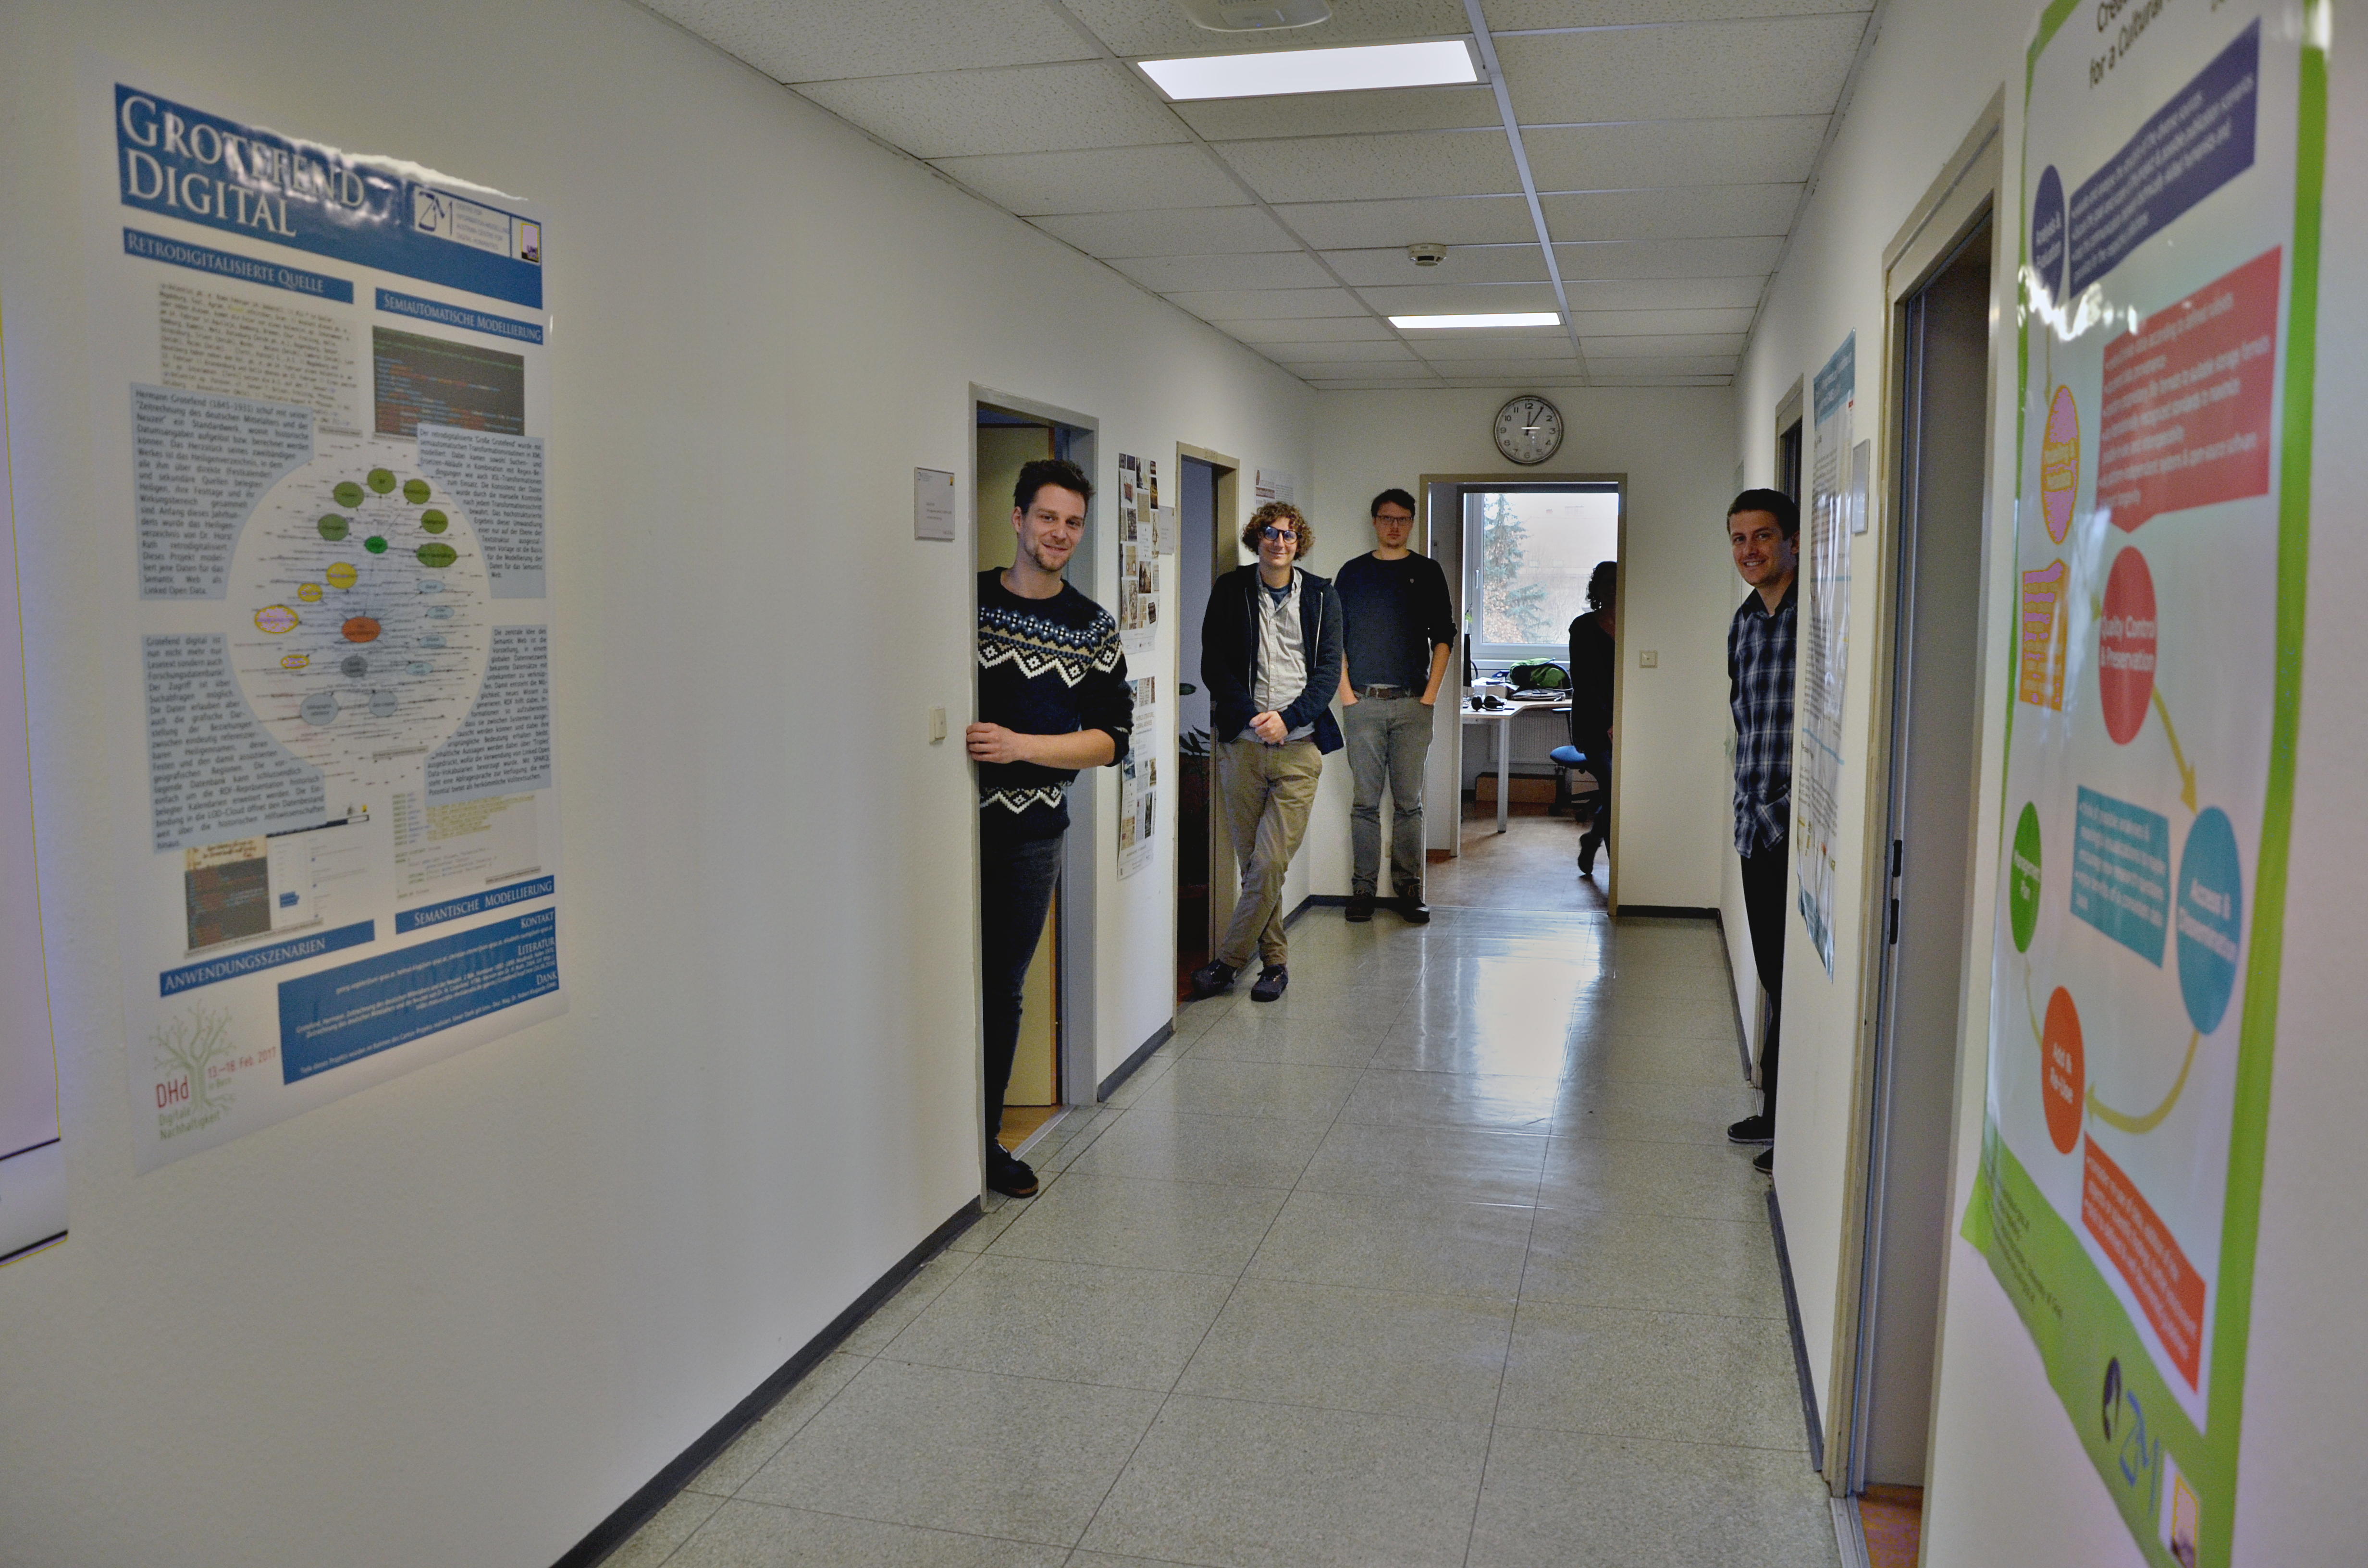
\includegraphics[height=10cm]{gang1.JPG}} ;}] (20,0) circle (5) ;

\draw[path picture={\node[anchor=center,fill=ZimBlue] at (path picture bounding box.center){\hspace{-4cm}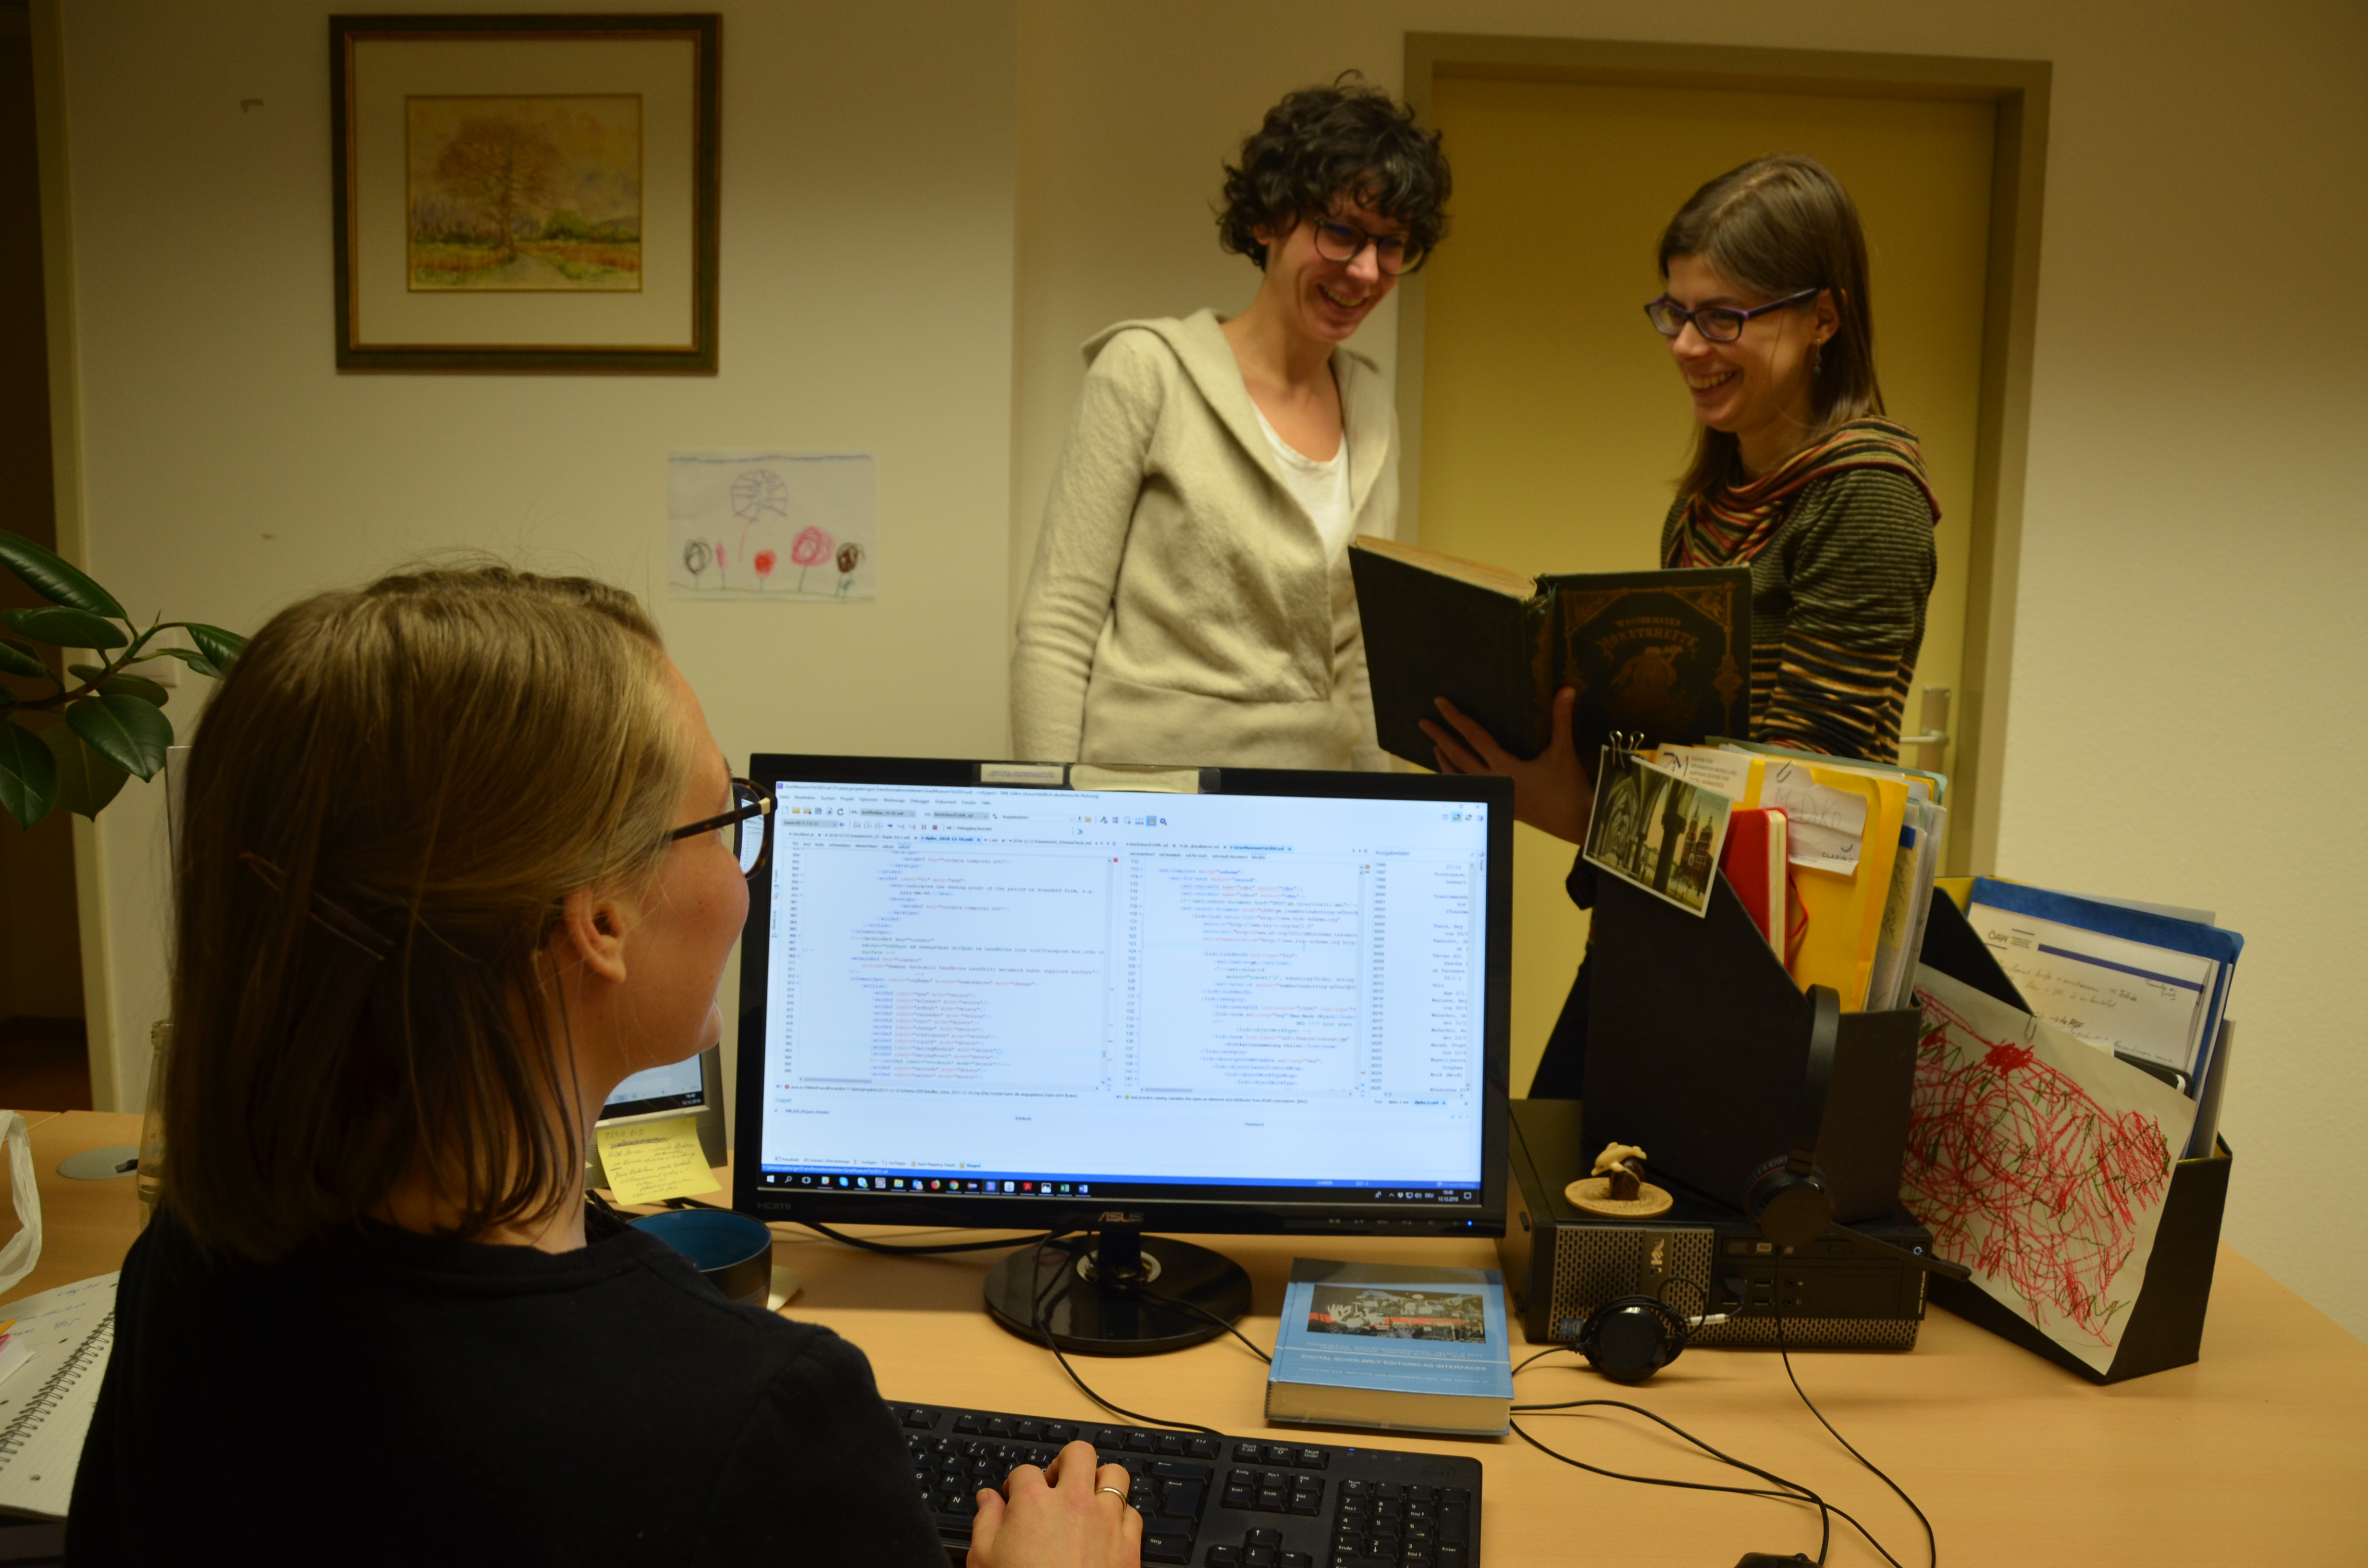
\includegraphics[height=13cm]{DSC_0131.JPG}} ;}] (14,8) circle (5) ;

\draw[path picture={\node[anchor=center,fill=ZimBlue] at (path picture bounding box.center){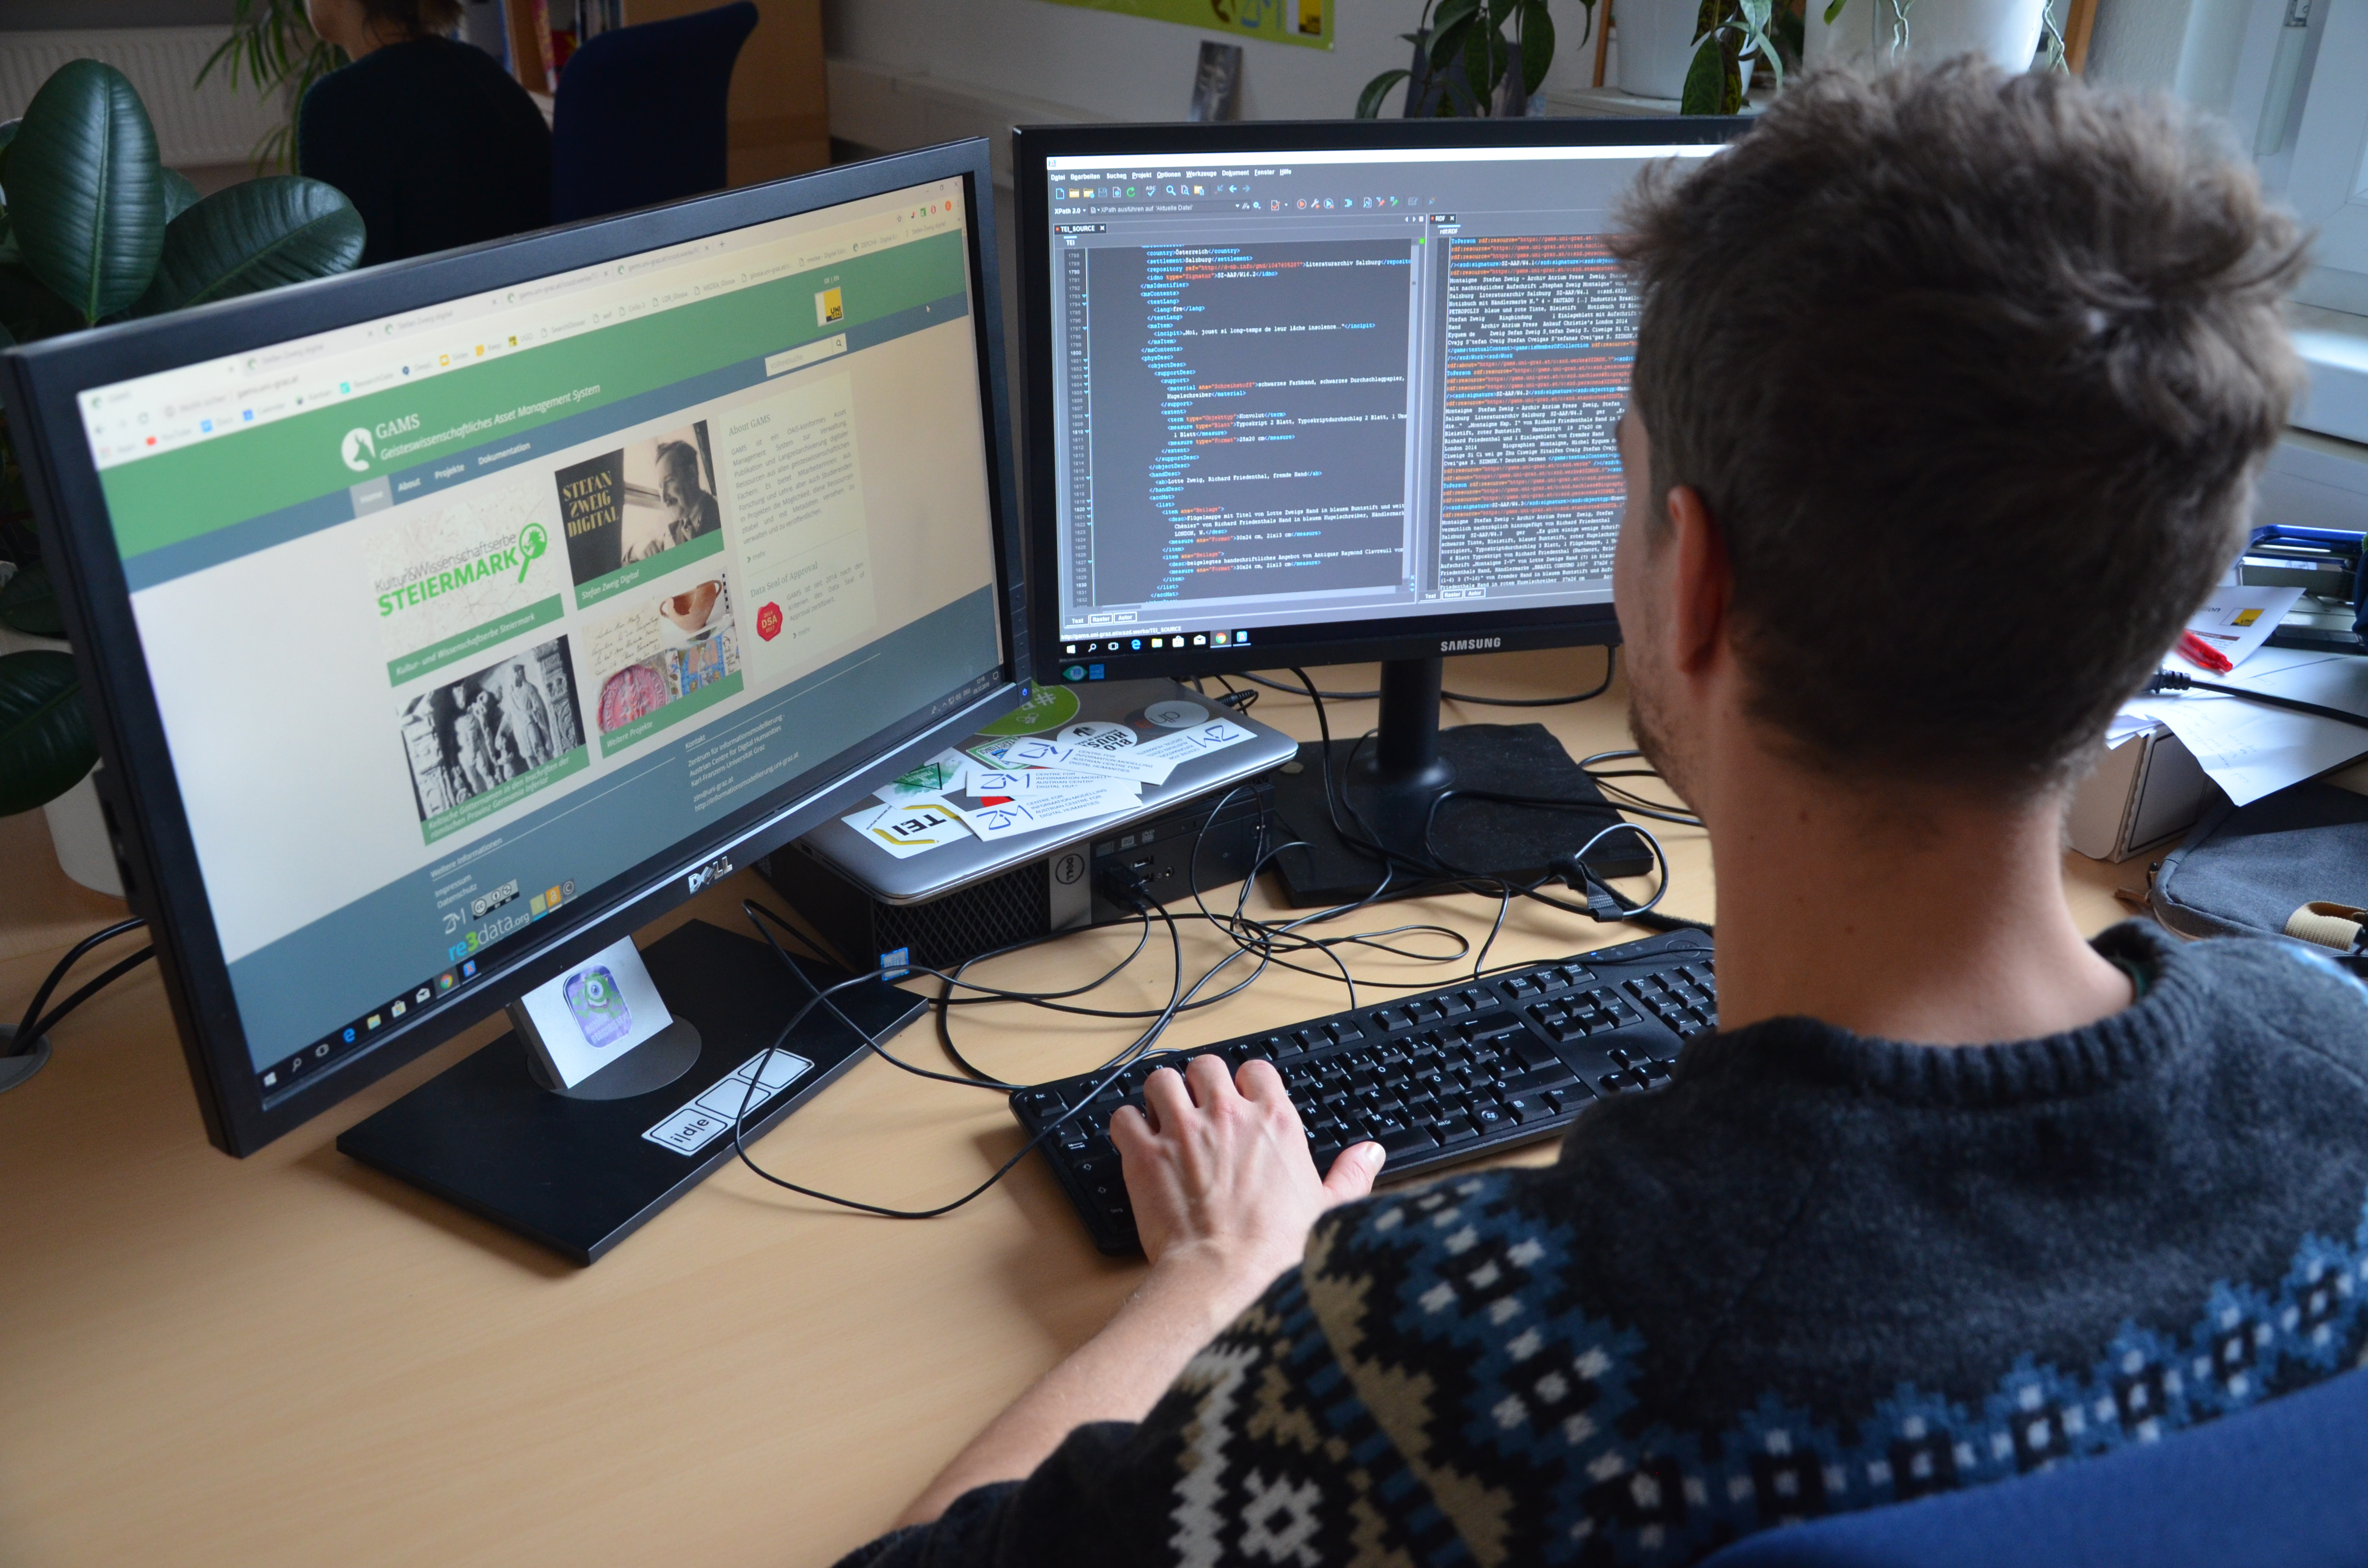
\includegraphics[height=13cm]{bildschirm2.JPG}} ;}] (9,19) circle (5) ;

}

\end{columns}
\begin{columns}
 \column{0.6}
    \block{}{
 \vspace{-1cm}   
\coloredbox[width=0.45\textwidth,bgcolor=GamsGreen!10,fgcolor=ZimBlue,framecolor=GamsGreen!10]{Kontakt.xml
\lstinputlisting{zim.xml}
}
}   
    
    \column{0.27}
        \block{}{
\vspace{-1cm}
		\bubblediagram{{\color{white}\textbf{Schwer-} \\\color{white}\textbf{punkte}},  Digital\\ Cultural\\Heritage, \textbf{XML}, {Digitale \\ Archive},\textbf{XSL},{Digital \\ Scholarly \\Editions}, Web\\Apps, Semantic\\ Web,\textbf{TEI}}
		
		%\bubbleicon{\Huge\faBook}{Reading}{white}{\huge}


 }
    
\end{columns}


\draw[fill=ZimBlue,draw=ZimBlue,minimum width=\paperwidth] (-40cm,-35cm) -- ++(0,7cm) -- (\paperwidth,-35cm) --  cycle;


\node [above right,outer sep=0pt,minimum width=\paperwidth,minimum height=5cm,align=center,draw=ZimBlue,fill=ZimBlue](footer) at (bottomleft) {
\begin{minipage}{\textwidth}
\vspace{1cm}\hspace{2cm}\color{white}\Large\MakeUppercase{\textbf{Master}studium\textbf{Digitale}Geisteswissenschaften}\hfill
\includegraphics[width=0.07\textwidth]{gamsweiss.png}\hspace{2cm}
\includegraphics[width=0.07\textwidth]{ZIM_weiss.png}\hspace{2em}
\includegraphics[width=0.07\textwidth]{kfFarbe.jpg}\hspace{2em}\vspace{2cm}
\end{minipage}
};

\end{document}
